\documentclass[]{article}
\usepackage[utf8]{inputenc}
\usepackage{graphicx}
\usepackage{listings}

\begin{document}
\title{
Tree nursery \\
\small PHP homework
}
\author{Tóth Bence Tamás - NTHJMZ }
\date{29. September 2018}
\maketitle

\section{Topic}
\paragraph{} This program is about the management of a tree nursery.
I store the values listed below for every tree.
\begin{enumerate}
    \item id, does nothing for now.
    \item name, the type of the tree.
    \item height, measured in \textit{[m]}.
    \item home, the original location of the plant.
    \item price
    \item age
\end{enumerate}

\begin{figure}[h]
    \centering
    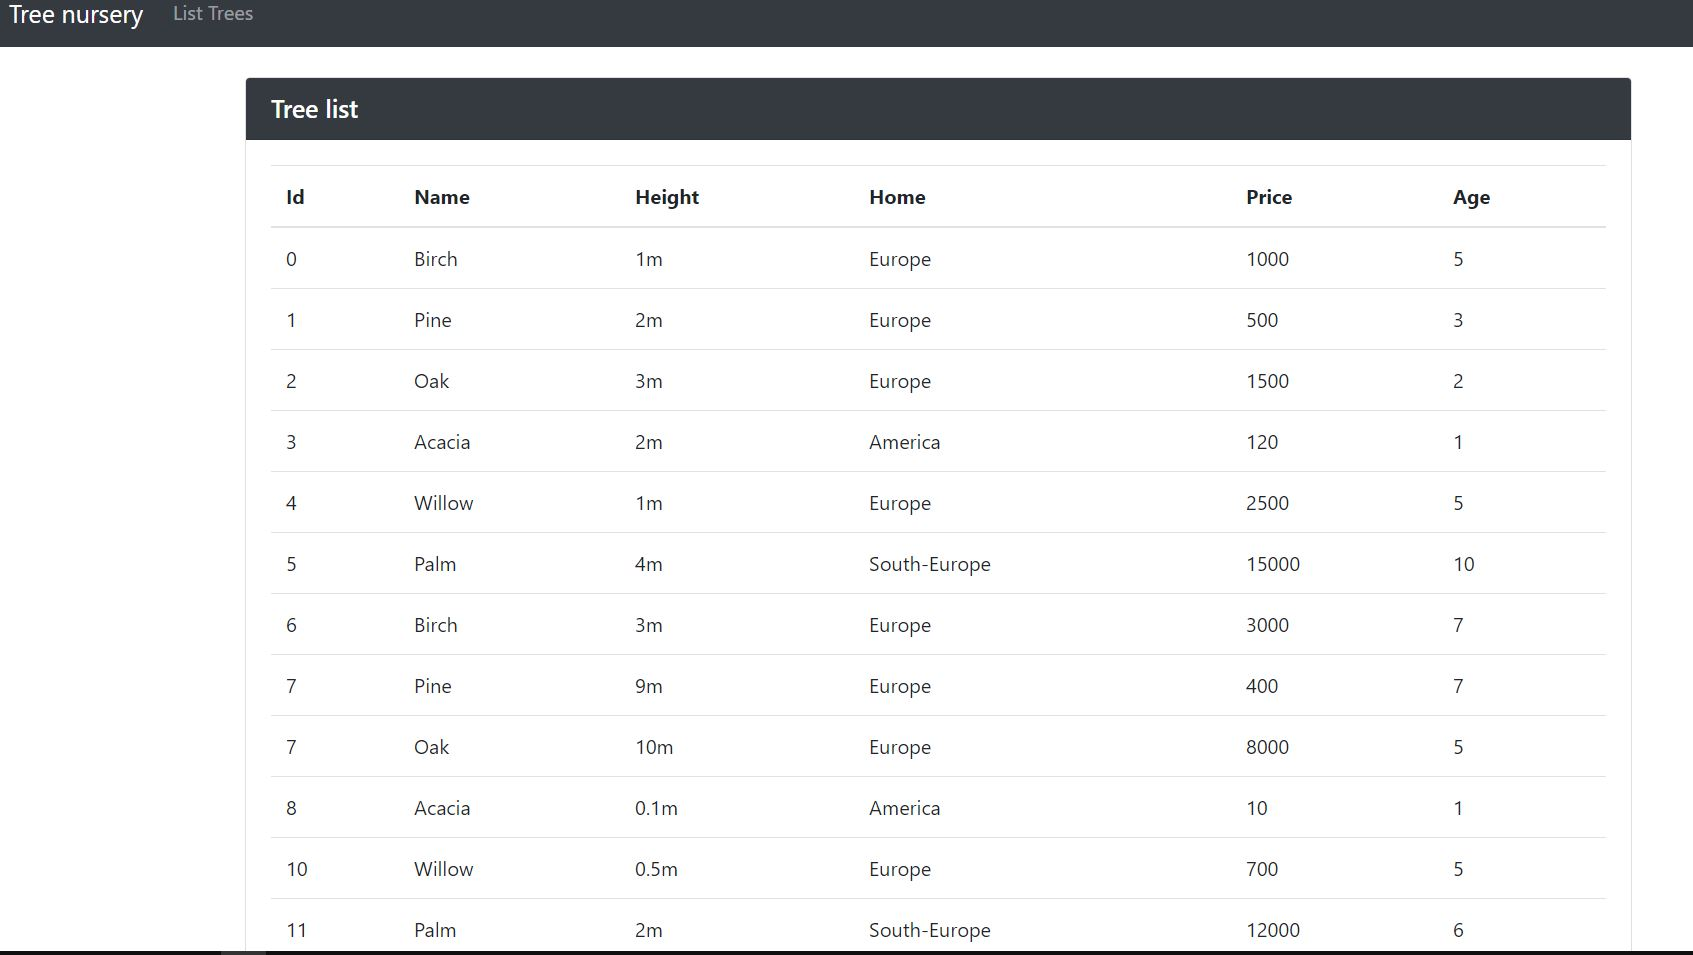
\includegraphics[width=0.9\textwidth]{treelist.JPG}
    \caption{List of original trees}
\end{figure}

\section{Questions}
\begin{enumerate}
    \item Which tree is the highest?
    \item Which tree is the oldest?
    \item How much 2 years old trees do we have?
    \item How much Pine trees do we have?
    \item How much is the total cost of our trees?
\end{enumerate}
\begin{figure}[h]
    \centering
    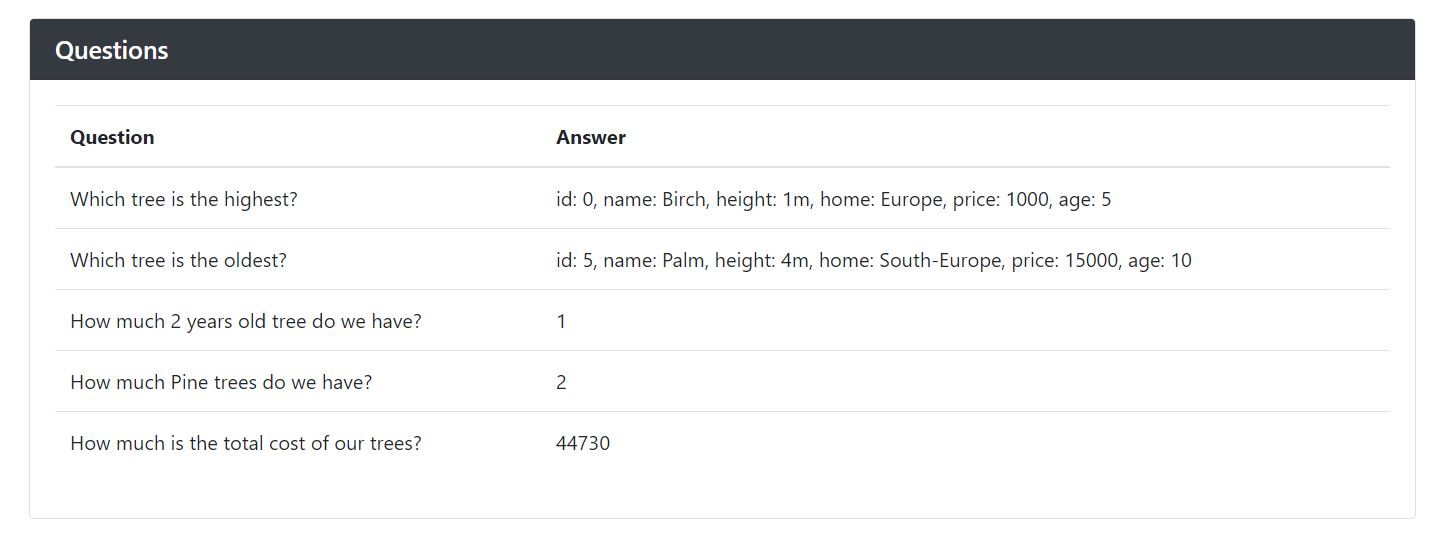
\includegraphics[width=\textwidth]{qalist.jpg}
    \caption{List of questions and answers}
\end{figure}

\section{Random entries}
\begin{figure}[h]
    \centering
    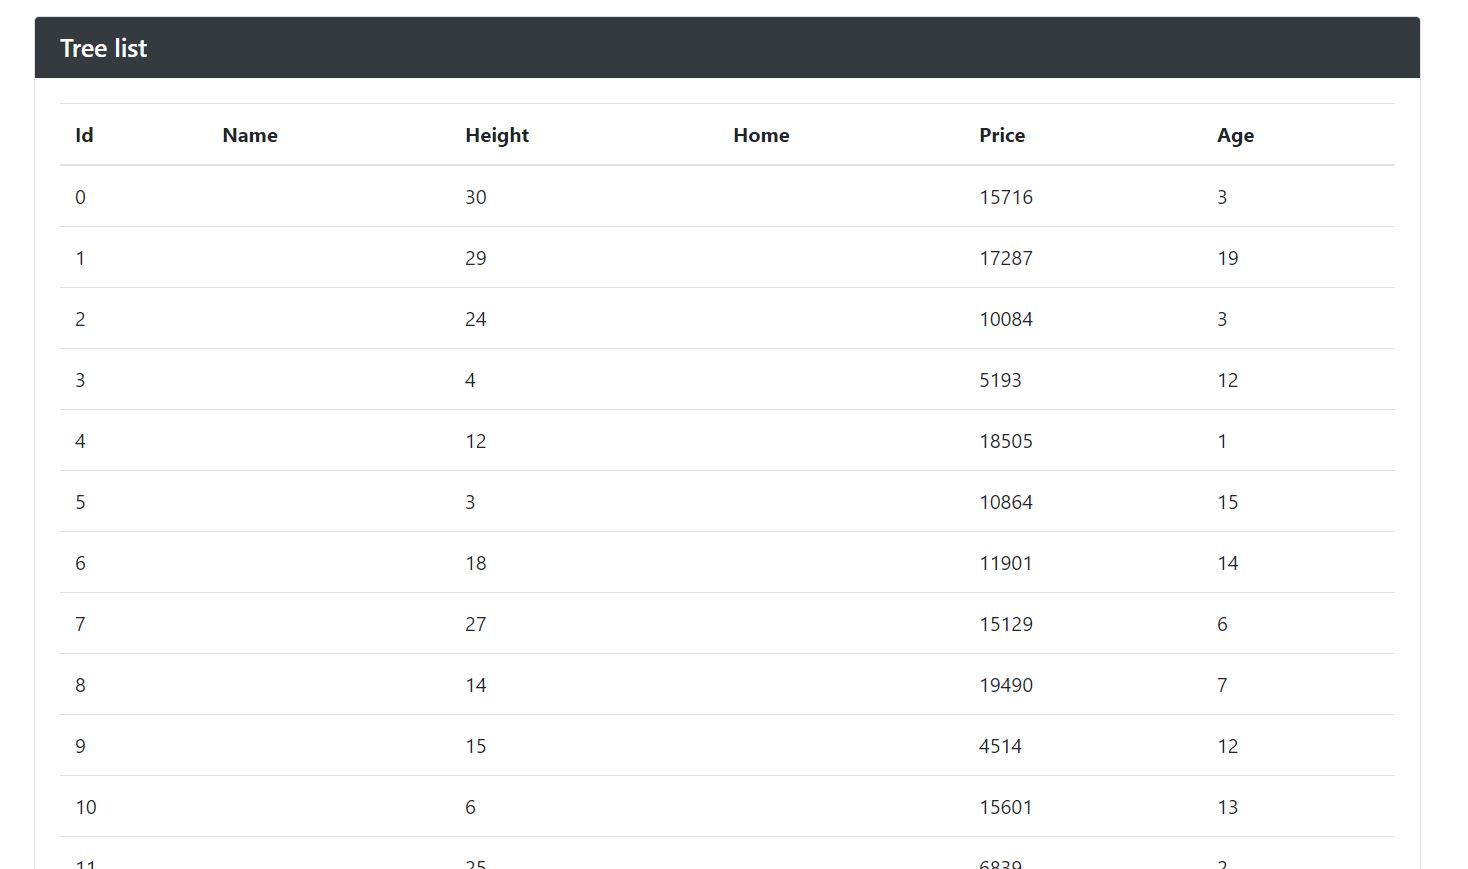
\includegraphics[width=\textwidth]{randomtrees.JPG}
    \caption{List of randomised entries}
\end{figure}

\section{Complex question}
\begin{enumerate}
    \item Union of the two lists.
    \item Intersection of the two lists.
    \item Difference (trees - random trees).
\end{enumerate}
\begin{figure}[h]
    \centering
    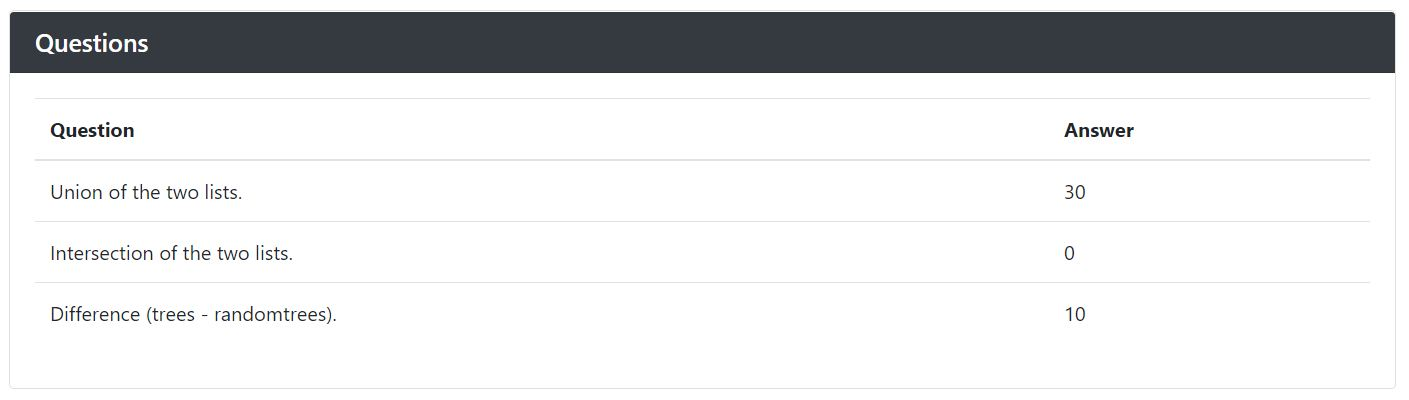
\includegraphics[width=\textwidth]{qa0.JPG}
    \caption{List of complex questions and answers}
\end{figure}
The numbers represent the number of elements in the results.
\begin{figure}[h]
    \centering
    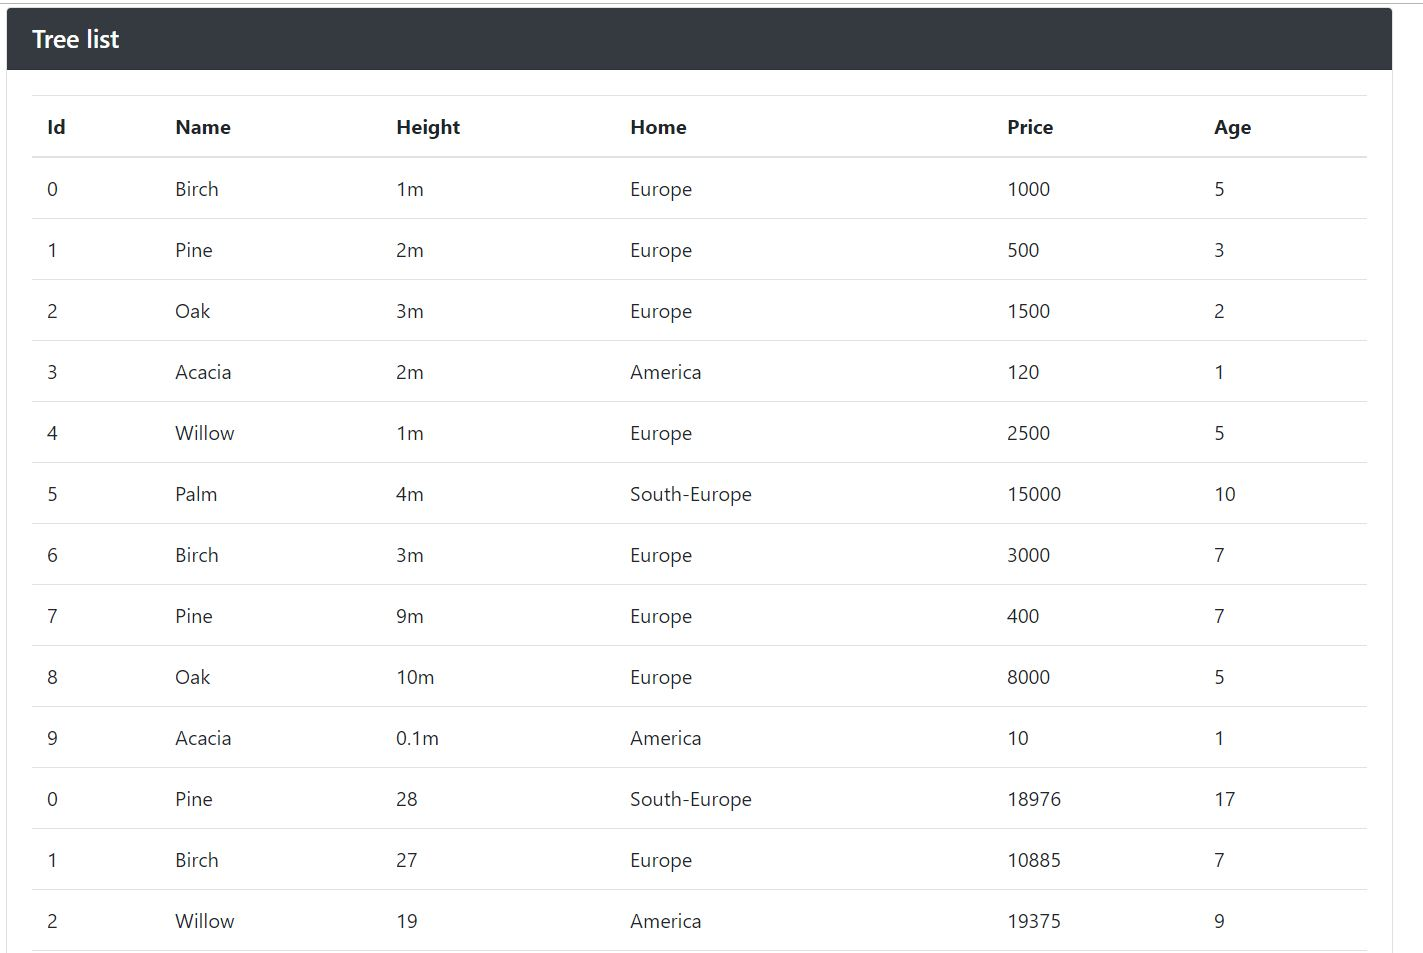
\includegraphics[width=\textwidth]{qa2.JPG}
    \caption{List of the union of the two lists}
\end{figure}
\paragraph{}
\newpage
The second complex question results in 0 elements because of the random factor, so it's table is not displayed.
\begin{lstlisting}[language=php, frame=single]
    
        
        <br/>
    
\end{lstlisting}

\begin{figure}[h]
    \centering
    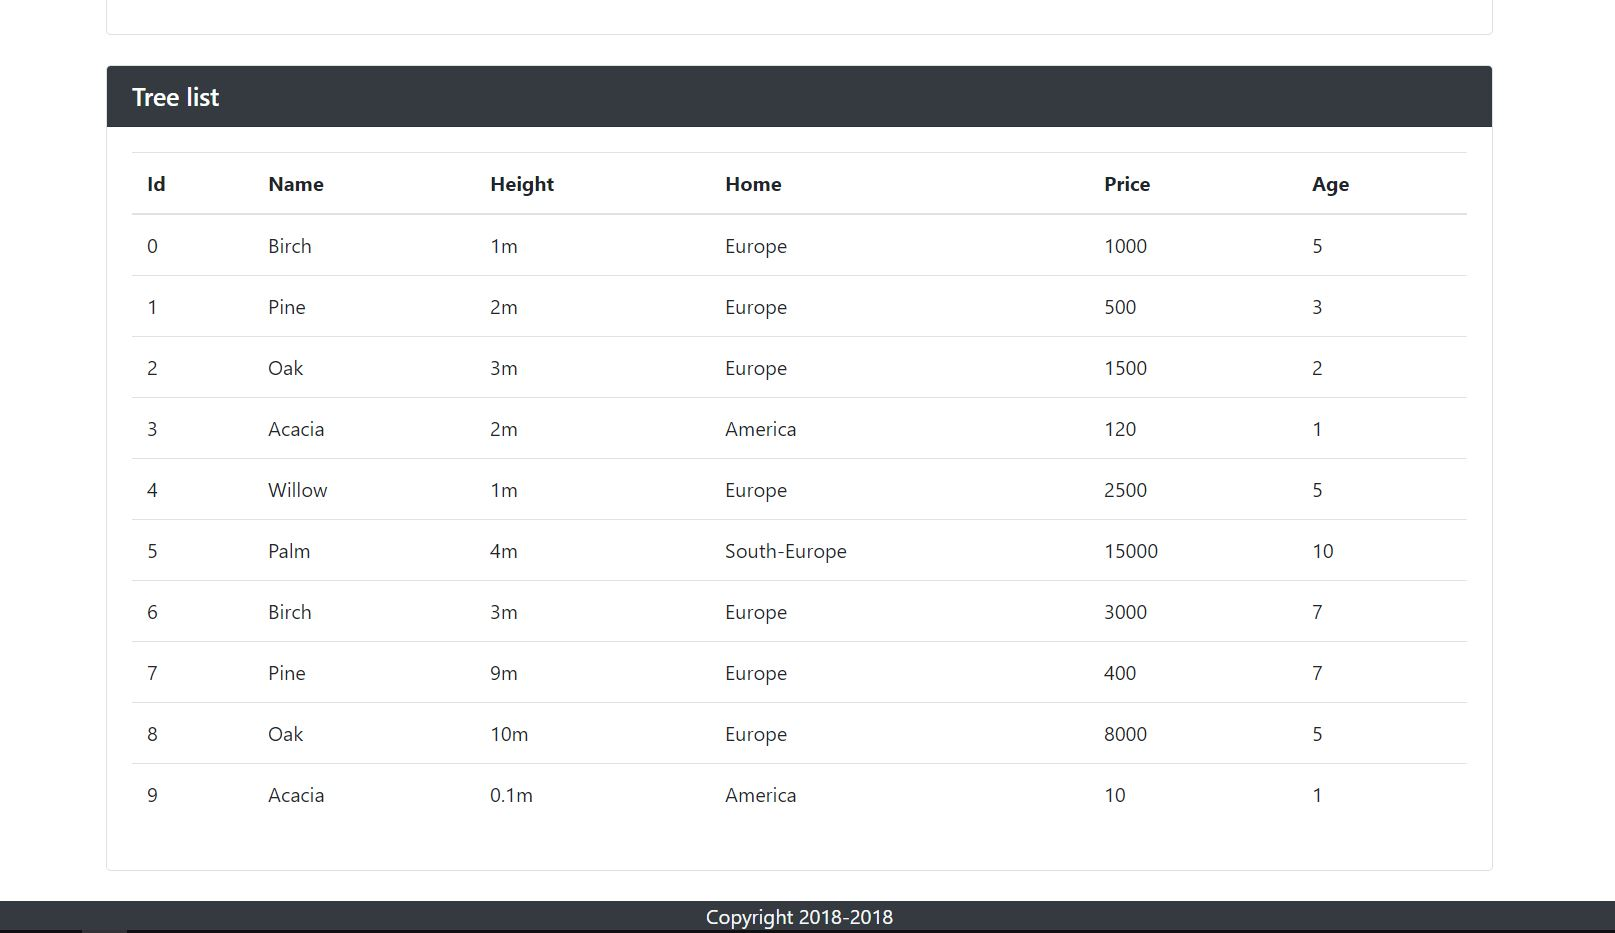
\includegraphics[width=\textwidth]{qa3.JPG}
    \caption{List of differences}
\end{figure}

\end{document}